\documentclass[11pt]{article}
\usepackage[letterpaper,margin=1in]{geometry}
\usepackage{amsmath,amssymb}
\usepackage{graphicx}
\usepackage{booktabs}
\usepackage{array}
\usepackage[font=small,labelfont=bf]{caption}
\usepackage[colorlinks=true,allcolors=blue]{hyperref}
\graphicspath{{bench/}}

\title{\textbf{A Living, Difficulty-Calibrated Benchmark\\for Virtual Cell Models}}
\author{}
\date{}

\begin{document}
\maketitle
\vspace{-2.5em}

% ---------------------------------------------------------------------------
\begin{abstract}
Virtual cell models are ranked by averaging a score over test cases, as if every
case were equally hard. They are not. In perturbation prediction, a model earns
credit on conditions where cells barely respond; in cell-type annotation, on cells of
the most common types; and the few cases that actually separate models are averaged
away. A fixed test set also loses value as models improve, and the field has no
agreed procedure for replacing it. We build a benchmark that treats every test case as
an item with a measured difficulty, as standardized tests do. It has two parts:
20,026 cells from a donor-held-out slice of Tabula Sapiens v2, where an item is passed
when a fixed linear classifier recovers the cell's type from a model's embedding; and
74,197 perturbation conditions from fourteen public screens, including the fifty-cell-line
Tahoe-100M drug atlas, where an item is passed when a model predicts the response
better than the average response of all other perturbations. Difficulties are
estimated with a one-parameter item response model from a pool of 20 to 30 deliberately
simple respondents per component (principal components, random projections, ridge
and nearest-neighbour regression, Gaussian processes, and their floors), so the scale is anchored to
methods that cannot have memorized the test data. The resulting map reproduces what
the field has found with raw scores and adds what raw scores hide: a quarter of the
perturbation conditions are passed by no method because the average response is
unbeatable on them; cell difficulty falls with how many training cells a type has;
and an scVI embedding sits a quarter of a logit below principal components on
held-out donors. Placing two learned models on the scale shows that a latent-space
model wins only when a drug has been observed in many cell lines. Finally, we quantify
maintenance: a model one logit above the best current respondent would retire half of
the annotation items and a quarter of the perturbation items, which fixes the rate at
which new hard items must be written.
\end{abstract}

% ---------------------------------------------------------------------------
\section{Dataset Composition and Statistics}
\label{sec:data}

\paragraph{Vocabulary.}
We borrow three words from item response theory~\cite{lord1980}, the framework behind standardized
tests. A \emph{respondent} is a model. An \emph{item} is one test case. A
\emph{response} is pass or fail. Each respondent has an ability $\theta$ and each
item a difficulty $b$, both on the same scale, and the probability that respondent
$j$ passes item $i$ is $\sigma(\theta_j-b_i)$ with $\sigma$ the logistic function.
The unit of the scale is a logit: one logit of extra ability multiplies the odds of
passing any item by $e\approx2.7$. Abilities and difficulties are estimated jointly
from the pass/fail matrix, so a model is credited more for passing hard items than
easy ones, and an item is called hard because strong models fail it, not because of
any prior notion of what should be hard. The bank has two components with different
items but the same response format.

\paragraph{Component A: representation.}
An item is one cell. A respondent is an embedding method, which maps a cell's
expression profile to a vector. The response is whether a multinomial logistic
regression, trained once on the embeddings of a separate training panel with fixed
settings, assigns the cell its annotated type. The classifier is identical for every
respondent, so a difference in responses is a difference in embeddings.

\paragraph{Component B: perturbation.}
An item is one experimental condition: a perturbation (a CRISPR target gene or a
compound) applied in one context (a cell line or a culture condition), at one dose
where doses vary. The cells of a condition are replicates, not items; the measured
response of an item is the mean log-normalized expression of its cells minus that of
matched control cells. A respondent predicts this response for conditions it has not
been trained on. We score a prediction by its Pearson correlation with the measured
response over the 2,000 most variable genes, and the item is passed when that
correlation exceeds the one obtained by a fixed reference: predicting, for every
condition, the average response of all training conditions in that context (the
\emph{mean shift}). The reference is chosen on purpose. Recent benchmarks~\cite{systema,perturbench,ahlmann2025} found that
this average matches deep models on standard metrics, because much of any response is
shared across perturbations; a pass therefore credits the perturbation-specific part
of a prediction and not the part every perturbation shares.

\paragraph{Sources.}
Component A uses Tabula Sapiens v2~\cite{tabulasapiens2}, 28 tissues and 23 donors with 10x data. Component B
uses thirteen screens from the scPerturb collection~\cite{scperturb} and the Tahoe-100M drug atlas~\cite{tahoe}
(Table~\ref{tab:compB}). All sources are public under CC0 or CC BY licences.

\begin{table}[t]
\centering
\small
\caption{Perturbation items by source. An item is a condition with at least 50
quality-passing cells and a matched control. ``Contexts'' are cell lines or culture
conditions. Tahoe-100M conditions are (compound, dose, cell line) triples; the Replogle
genome-wide screen is the largest genetic source. Cell counts are after quality filtering.}
\label{tab:compB}
\footnotesize
\begin{tabular}{@{}llrrrr@{}}
\toprule
Dataset & Perturbation & Contexts & Perturbations & Items & Cells \\
\midrule
Tahoe-100M & compound, 3 doses & 50 & 379 & 53,972 & 95.6M \\
Replogle 2022, K562 genome-wide & CRISPRi & 1 & 9,326 & 9,326 & 1.97M \\
Srivatsan 2020 (sciPlex3) & compound, 4 doses & 3 & 188 & 2,423 & 762k \\
Replogle 2022, K562 essential & CRISPRi & 1 & 1,832 & 1,832 & 303k \\
Nadig 2024, Jurkat & CRISPRi & 1 & 1,815 & 1,815 & 245k \\
Replogle 2022, RPE1 & CRISPRi & 1 & 1,611 & 1,611 & 225k \\
Nadig 2024, HepG2 & CRISPRi & 1 & 1,061 & 1,061 & 104k \\
McFarland 2020 & compound, 7 doses & 196 & 16 & 866 & 166k \\
Frangieh 2021 & CRISPR knockout & 3 & 229 & 669 & 216k \\
Norman 2019 & CRISPRa (single, double) & 1 & 236 & 236 & 111k \\
Tian 2021, neurons & CRISPRi & 1 & 183 & 183 & 32k \\
Adamson 2016 & CRISPRi & 1 & 87 & 87 & 63k \\
Tian 2019, iPSC & CRISPRi & 1 & 81 & 81 & 29k \\
Tian 2019, neurons & CRISPRi & 1 & 35 & 35 & 8k \\
\midrule
Total & & & & 74,197 & 99.9M \\
\bottomrule
\end{tabular}
\end{table}

\paragraph{Representation panel.}
Donors are split before anything else: 21 donors supply a training panel of 146,800
cells and 2 donors supply the test items, so no donor appears on both sides and the
classifier cannot learn donor identity as a stand-in for cell type. We call each (tissue, cell type, donor) combination a \emph{stratum}; within each stratum
we keep at most 200 training and 50 test cells and drop strata with fewer than 20 cells. The result is 20,026 test items in 433 strata
across 28 tissues and 102 cell types (159 types appear in training). Immune cells are
58\% of the items, stromal 18\%, epithelial 13\%, endothelial 10\%. The 844 test cells
whose type is absent from training are kept in the panel but not scored.

\paragraph{Perturbation items.}
Every screen is mapped to one schema (perturbation, target genes, modality, context,
dose, time, control flag); cells with fewer than 500 counts or 200 detected genes are
removed; and the per-condition mean is computed in one pass over the raw count
matrix. For Tahoe-100M this pass streams 95.6 million cells from the public parquet
files and reduces them to 56,827 (compound, dose, cell line) conditions, of which
53,972 have at least 50 cells. Median cells per item range from 74 (Nadig HepG2) to
1,363 (Tahoe-100M). Each item carries covariates for later analysis: cell count, an
effect-size measure (the Euclidean norm of the response), the target gene or the
compound's chemical structure, and dose.

\paragraph{Difficulty distributions.}
Figure~\ref{fig:difficulty} shows the fitted difficulties. Three features determine
how the bank can be used.

\emph{The scale is wide.} Informative difficulties span about six logits in both
components (5th to 95th percentile: $-3.2$ to $2.6$ for cells, $-4.2$ to $1.6$ for
conditions), with standard deviations of 1.8 and 1.6. The abilities of the classical
pool occupy the shaded band in each panel. The bank already holds items well above
its best respondent, which is the stock a living benchmark draws on as models
improve.

\emph{A fifth of the items are off the scale today.} 2,270 cells (11\%) are labelled
correctly by no respondent, and 4,664 conditions (23\%) are passed either by all
respondents (88) or by none (4,576). The latter are conditions on which the mean
shift is the best prediction any method in the pool can make. They are hard in the
useful sense and stay in the bank, but they carry no information about the current
ranking and have no finite difficulty until some model passes them.

\emph{Datasets differ by more than their items.} On the pooled perturbation scale the
mean difficulty by dataset ranges from $-1.7$ (Norman, where every double
perturbation has both of its singles in training) to $+1.0$ (Tian 2021 neurons), a
spread of 2.7 logits against a within-dataset standard deviation of about 1.5. A
single pooled scale is therefore a first approximation. The K562 screens share
thousands of target genes, and those shared conditions are the natural anchors for
linking datasets in the next release.

\paragraph{What makes an item hard.}
Difficulty tracks the covariates the design predicts. For cells, difficulty falls
with the number of training cells of the same type (Spearman $\rho=-0.35$ over
17,756 items; $-0.47$ at the stratum level) and, more weakly, with sequencing depth
($\rho=-0.10$). The hardest types are sibling immune states (activated versus naive
CD8 T cells, gamma-delta T cells, innate lymphoid cells, intermediate monocytes) and
stromal types that share a lineage (mural and muscle cells, mesenchymal stem cells).
For conditions the sign is the reverse of what a raw metric would give: difficulty
rises weakly with effect size ($\rho=+0.15$ pooled; $+0.18$ in the genome-wide K562
screen, $+0.25$ in RPE1). Large responses are the ones the mean shift already
captures, so beating it there is hard, while small responses are close to coin
flips. The pass rule thus changes what difficulty means; we keep the continuous
scores so that a graded fit can be run alongside the binary one.

\begin{figure}[t]
\centering
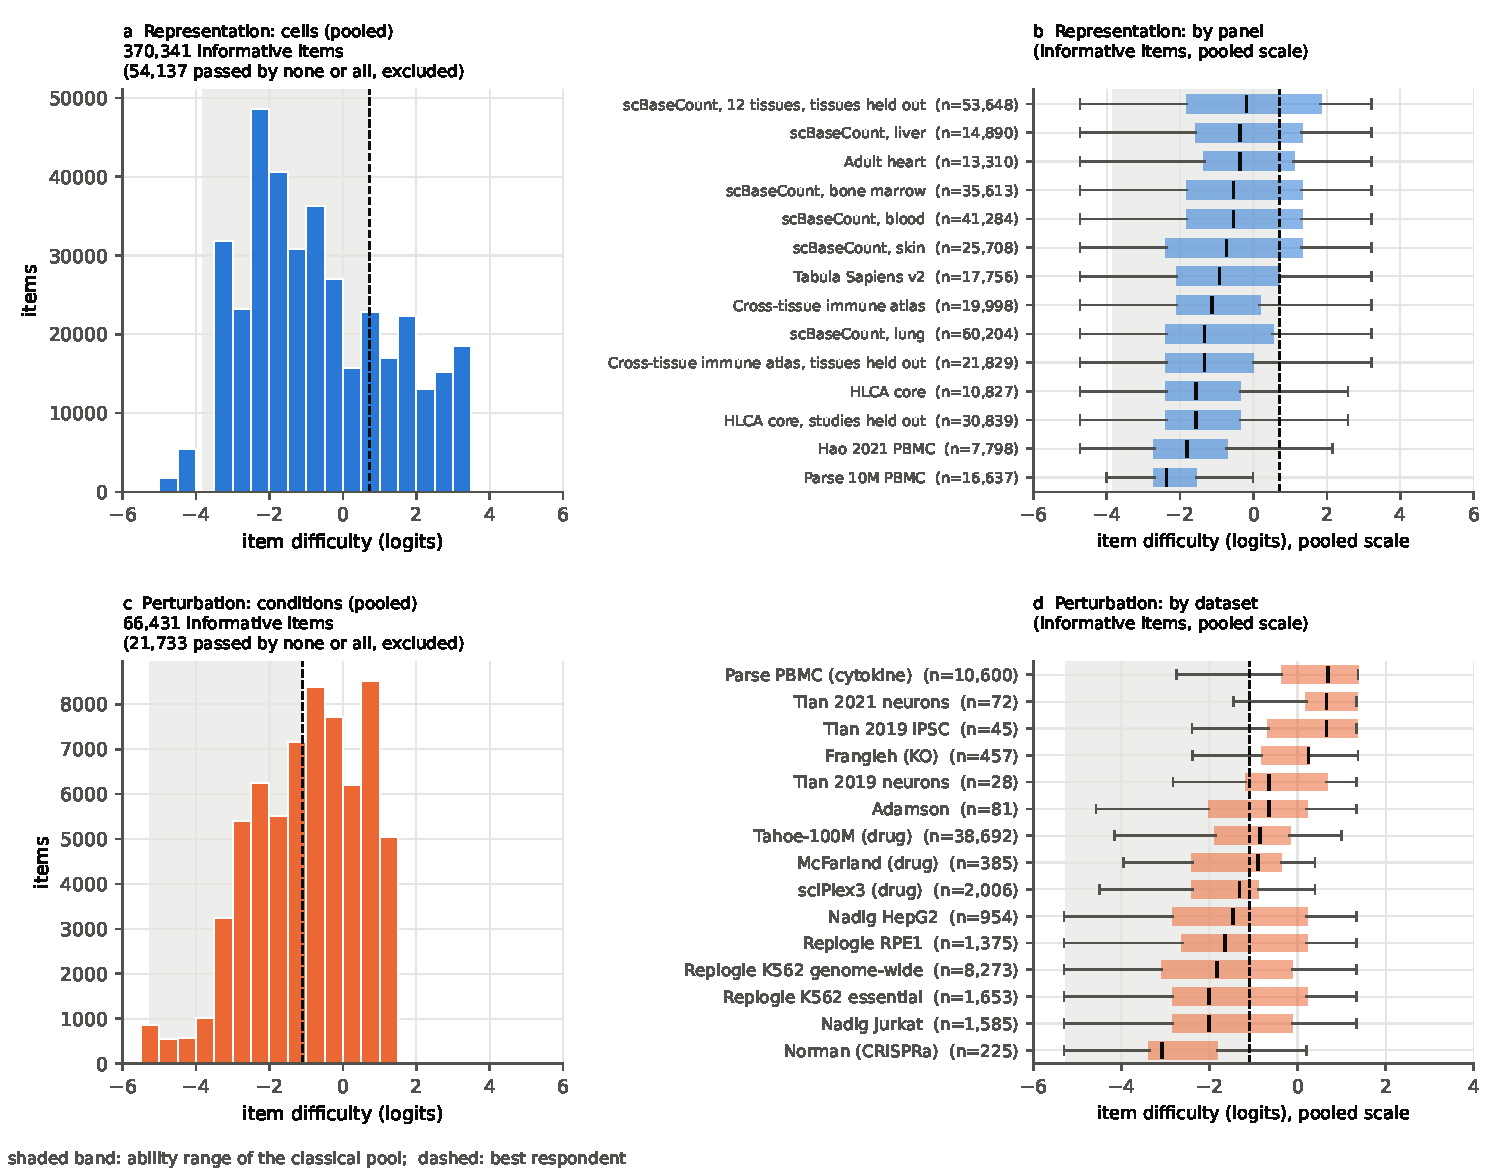
\includegraphics[width=0.92\textwidth]{fig_difficulty.pdf}
\caption{Item difficulty on the logit scale. (a) Representation items (cells). (b) The same cells grouped into
\emph{strata}, one stratum per (tissue, cell type, donor) combination, so that each
stratum is one item answered $k$ times correctly out of its $n$ cells (a binomial fit);
this removes the dependence between cells of the same type from the same donor. (c) Perturbation
conditions pooled across datasets and (d) the same conditions by dataset (boxes span the
interquartile range, whiskers the 5th to 95th percentile). The shaded band is the ability
range of the classical pool and the dashed line its best respondent. An item is
``informative'' when at least one respondent passes it and at least one fails it.}
\label{fig:difficulty}
\end{figure}

% ---------------------------------------------------------------------------
\section{Model Evaluation}
\label{sec:eval}

\paragraph{Why simple models come first.}
A difficulty scale is only as trustworthy as the respondents that define it. We
calibrate with methods that are cheap, transparent, and cannot have seen the test
data during pretraining. Within each family we vary one capacity setting so that
abilities spread out in a known order, and we include several families so that items
which one family passes and another fails become visible. Floors (random embeddings,
random shifts, predicting no change) pin the bottom of the scale. Pretrained
foundation models are placed on the scale afterwards; this is the only order in which
their abilities can be read separately from their exposure to the test data.

\paragraph{Respondents.}
Component A has 27 classical respondents and three settings of scVI~\cite{scvi}, a variational
autoencoder for single-cell counts: principal components (PCA) with 4 to 256
components, Gaussian random projections, kernel (Nystr\"om) features, non-negative
matrix factorization, independent components, soft cluster memberships from a
Gaussian mixture, a floor that sees only sequencing depth, and random embeddings.
Component B has 18 classical respondents per genetic screen: predicting no change,
the mean shift, the mean shift with a forced change at the target gene, random
shifts, nearest-neighbour averaging ($k=1,5,20$), ridge regression from perturbation
features into a low-dimensional basis of the training responses (two ranks, two
penalties), Gaussian-process regression (two kernel widths), and the same ridge and
nearest-neighbour models trained on 30\% and 10\% of the training items. Screens with
several contexts add a low-rank completion of the perturbation-by-context response
matrix (ranks 2, 5, 10). Genetic items are represented by a 64-dimensional embedding
of the target gene learned from control cells only; compounds by Morgan fingerprints
of their chemical structure~\cite{morgan}. The learned model for component B is scGen~\cite{scgen}, a
variational autoencoder that predicts a perturbation in a new context by adding, in
latent space, the shift it observed for that perturbation in other contexts. We
re-implemented it with its published architecture.

\paragraph{Splits.}
Perturbation respondents are evaluated out of fold: perturbations are divided into
five folds, each respondent is trained on four and predicts the fifth, and every
condition therefore receives a prediction from a model that never saw its
perturbation. Screens with several contexts are additionally split over
(perturbation, context) pairs, so that a perturbation seen in some contexts must be
predicted in a new one. Representation respondents are fit on the training panel and
scored on the donor-held-out test panel. All respondents share the same folds, panel,
classifier, and metrics.

\paragraph{Fit.}
We fit the one-parameter logistic model by joint maximum likelihood with a weak
Gaussian prior on abilities and difficulties, which fixes the location of the scale
and keeps items that everyone passes or fails finite. Standard errors come from the
observed Fisher information. On synthetic data with 80 respondents and 2,000 items at
30\% missingness, the fit recovers abilities with correlation 0.998 and difficulties
with correlation 0.969, with an error equal to the reported standard error. For cells
we report a cell-level fit and a stratum-level binomial fit. Each respondent also gets
an \emph{outfit} statistic, a mean squared standardized residual: values near 1 mean
the respondent's passes and fails follow the model, values above 2 flag a pattern the
one-parameter model does not describe.

\begin{table}[t]
\centering
\small
\caption{Representation respondents on the cell-level scale (20,026 items). \emph{Ability}
is the item-response estimate in logits (higher is better) with its standard error
\emph{SE}; \emph{Accuracy} is the plain fraction of test cells labelled correctly, shown
for comparison with conventional reporting; \emph{Outfit} is the fit statistic defined in
the text (near 1: the respondent's pattern of passes and fails is what the model
predicts; above 2: it is not). The full ladder of 30 respondents is in the supplement.}
\label{tab:abilA}
\begin{tabular}{@{}lrrrr@{}}
\toprule
Respondent & Ability (logit) & SE & Accuracy & Outfit \\
\midrule
PCA, 128 components & 0.98 & 0.02 & 0.65 & 0.55 \\
PCA, 256 components & 0.94 & 0.02 & 0.65 & 0.68 \\
Nystr\"om kernel features, 256 & 0.85 & 0.02 & 0.64 & 0.53 \\
Independent components, 64 & 0.81 & 0.02 & 0.64 & 0.39 \\
PCA, 64 components & 0.81 & 0.02 & 0.64 & 0.40 \\
scVI, 30 latent, no batch correction & 0.74 & 0.02 & 0.63 & 0.73 \\
PCA, 32 components & 0.55 & 0.02 & 0.61 & 0.46 \\
Non-negative factorization, 64 & 0.49 & 0.02 & 0.60 & 0.68 \\
scVI, 30 latent, corrected for tissue & 0.47 & 0.02 & 0.60 & 0.79 \\
Random projection, 128 dimensions & 0.35 & 0.02 & 0.58 & 0.85 \\
scVI, 10 latent, corrected for tissue & 0.10 & 0.02 & 0.55 & 0.73 \\
PCA, 16 components & $-0.11$ & 0.02 & 0.53 & 0.63 \\
Gaussian-mixture memberships, 100 & $-0.57$ & 0.02 & 0.46 & 0.72 \\
PCA, 8 components & $-1.34$ & 0.02 & 0.36 & 1.04 \\
PCA, 4 components & $-2.14$ & 0.02 & 0.25 & 1.65 \\
Sequencing depth only & $-2.97$ & 0.02 & 0.16 & 2.00 \\
Random embedding & $-4.14$ & 0.03 & 0.07 & 4.25 \\
\bottomrule
\end{tabular}
\end{table}

\begin{table}[t]
\centering
\small
\caption{Abilities on the pooled perturbation scale (20 respondents, 20,225 conditions from
the thirteen scPerturb screens; Tahoe-100M is reported separately in the supplement).
Columns as in Table~\ref{tab:abilA}, except that \emph{Pass rate} is the fraction of
conditions on which the respondent beat the mean shift. Low-rank completion ran only on the
three multi-context screens, so its ability is not comparable to the rest. ``30\% train''
marks the training-fraction ladder.}
\label{tab:abilB}
\begin{tabular}{@{}lrrrr@{}}
\toprule
Respondent & Ability (logit) & SE & Pass rate & Outfit \\
\midrule
Low-rank completion (ranks 2, 5, 10; 3 screens only) & 0.21 & 0.05 & 0.34 & 0.47 \\
Ridge, 10-dim basis, strong penalty & $-0.31$ & 0.02 & 0.50 & 0.64 \\
Ridge, 10-dim basis, weak penalty & $-0.37$ & 0.02 & 0.49 & 0.62 \\
Gaussian process, wide kernel & $-0.39$ & 0.02 & 0.49 & 0.79 \\
Ridge, 50-dim basis, strong penalty & $-0.42$ & 0.02 & 0.49 & 0.53 \\
Ridge, 50-dim basis, weak penalty & $-0.50$ & 0.02 & 0.48 & 0.53 \\
Gaussian process, narrow kernel & $-0.67$ & 0.02 & 0.45 & 0.81 \\
Ridge, 50-dim basis, 30\% train & $-0.89$ & 0.02 & 0.42 & 0.85 \\
Nearest neighbours, $k=20$ & $-1.33$ & 0.02 & 0.36 & 0.76 \\
Ridge, 50-dim basis, 10\% train & $-1.36$ & 0.02 & 0.36 & 0.92 \\
Nearest neighbours, $k=20$, 30\% train & $-1.42$ & 0.02 & 0.35 & 0.80 \\
Nearest neighbours, $k=5$ & $-1.69$ & 0.02 & 0.31 & 0.68 \\
Nearest neighbours, $k=1$ & $-1.96$ & 0.02 & 0.28 & 0.68 \\
Random shift (two seeds) & $-2.18$ & 0.02 & 0.23 & 0.91 \\
No change & $-2.40$ & 0.02 & 0.21 & 0.56 \\
Mean shift with forced on-target change & $-3.31$ & 0.03 & 0.12 & 4.57 \\
\bottomrule
\end{tabular}
\end{table}

\paragraph{The ladders behave as ladders.}
Ability rises with capacity in every family that has a capacity setting. PCA climbs
from $-2.14$ at 4 components to $0.98$ at 128 and flattens at 256
(Table~\ref{tab:abilA}). Random projections sit 0.6 to 1.4 logits below PCA at the
same dimension, which separates the value of ordering directions by variance from the
value of a linear subspace as such. In component B the training-fraction ladder is
ordered correctly in every one of the fourteen screens. The floors land where floors
should: random shifts, no change, and random embeddings are the bottom three of their
tables, and the random embedding's outfit of 4.3 flags it, correctly, as a guesser.
These checks are what justify reading the rest of the scale.

\paragraph{The mean shift is the respondent to beat.}
Ranked by raw Pearson correlation, the best method in seven of the thirteen
scPerturb screens is the mean shift itself or its on-target variant, which differs
from it at a single gene; this reproduces the finding of Systema~\cite{systema} and PerturBench~\cite{perturbench} under
a different protocol. The item view adds the distribution behind that average: 4,576
conditions (23\%) are passed by no respondent, and in the Tian 2021 neuronal screen
that fraction reaches two thirds. The feature-based families (ridge, Gaussian
process) pass about half of all conditions, which places them two logits above the
floors but within 0.4 logits of one another; with item standard errors of 0.6 logits,
that is the resolution the current pool affords. The one clear exception is Norman,
where nearest neighbours and the Gaussian process lead by a wide margin because every
double perturbation has both of its singles in training.

\paragraph{A learned embedding does not beat the PCA ladder on held-out donors.}
scVI's best setting (30 latent dimensions, no batch correction) has ability 0.74,
between PCA with 64 and 32 components and a quarter of a logit below PCA with 128.
Correcting for tissue as a batch variable lowers ability to 0.47, because tissue
carries type information that the classifier would otherwise use. These placements
agree with reports that parameter-free pipelines match learned representations on
annotation~\cite{kedzierska2025,souza2026}, and they are unremarkable in a second way: scVI's outfit of 0.7 to 0.8
says it behaves like an ordinary point on the scale rather than a specialist.

\paragraph{A learned perturbation model wins only when a drug has many contexts.}
scGen's result depends on how many contexts a perturbation has been observed in
(Table~\ref{tab:scgen}). On McFarland, where 16 compounds are profiled across 196
cell lines, scGen passes 81\% of items, has ability $+2.75$, and is the only
respondent in the bank that beats the mean shift on most items of a screen. On
sciPlex3 and Frangieh, with three contexts each, it falls below the mean shift on raw
correlation and below the low-rank completion on the scale. Transfer through a learned
latent space thus pays off in proportion to the contexts available, which is the
regime Tahoe-100M provides with fifty cell lines. Because scGen cannot predict a
perturbation it has never seen, it is placed per screen in the unseen-context setting
rather than on the pooled scale.

\begin{table}[t]
\centering
\small
\caption{scGen in the unseen-context setting. ``Raw'' is the mean Pearson correlation on the
2,000 most variable genes, with the mean shift's value in parentheses. Rank is among the
respondents that ran on that screen.}
\label{tab:scgen}
\begin{tabular}{@{}lrrrl@{}}
\toprule
Screen & Contexts & Raw (mean shift) & Ability (rank) & Best respondent \\
\midrule
McFarland 2020 & 196 & 0.53 (0.32) & $+2.75$ (1 of 9) & scGen \\
Srivatsan 2020 (sciPlex3) & 3 & 0.13 (0.26) & $-1.76$ (4 of 9) & low-rank, rank 10 \\
Frangieh 2021 & 3 & 0.18 (0.32) & $-2.77$ (10 of 22) & low-rank, rank 5 \\
\bottomrule
\end{tabular}
\end{table}

\paragraph{What a misfit looks like.}
One respondent fails the fit statistic: the mean shift with a forced on-target change
has outfit 4.6. It ties the mean shift exactly unless the target gene is among the
scored genes, and a tie counts as a fail, so its passes concentrate on an
idiosyncratic subset of items. We keep it as a diagnostic and exclude it from any
reading of the ladder. The stratum-level binomial fit for cells shows a second kind
of misfit: respondent outfits of 3 to 10, which means that cells within a stratum are
not interchangeable trials. The stratum fit orders respondents exactly as the cell
fit does, but its standard errors (0.07) are too small, and a model with a per-stratum
random effect is the correct replacement.

\paragraph{How many items would today's best models retire?}
A benchmark stays informative only while its items sit near the abilities being
measured; an item that a model passes with probability 0.95 or more has essentially
nothing left to say about that model. We therefore ask how much of the bank a
stronger model would retire (Figure~\ref{fig:retire}). A model exactly as able as the
best current respondent already retires 26\% of the informative cell items and 13\% of
the conditions. In a pilot of the same annotation protocol on three smaller atlases,
the strongest pretrained foundation model sat about one logit above PCA. A model one
logit above the best respondent here would retire 51\% of the cell items and 25\% of
the conditions, leaving 6,034 cells and 6,745 conditions inside its informative window
(within two logits of its ability). Two logits above retires 66\% and 57\%; four logits
exhausts the bank, with 811 cells and no conditions left in the window. Perturbation
items degrade more slowly, because their difficulties are spread over a wider range
and because the 4,576 conditions that no respondent passes only come into play as
models improve. The practical content is a writing schedule. The maintenance
analysis in our companion paper~\cite{companion} shows that a benchmark keeps its resolution only when
new hard items arrive at least as fast as the field moves; at the rates above, a bank
that loses half its annotation items per logit of progress must add items above the
current ceiling at the same pace. The yearly Virtual Cell Challenge releases~\cite{vcc2026} (300 to
10,000 held-out perturbations per cell line) and the announced Tahoe follow-on atlas
are the supply we plan the next rounds around.

\begin{figure}[t]
\centering
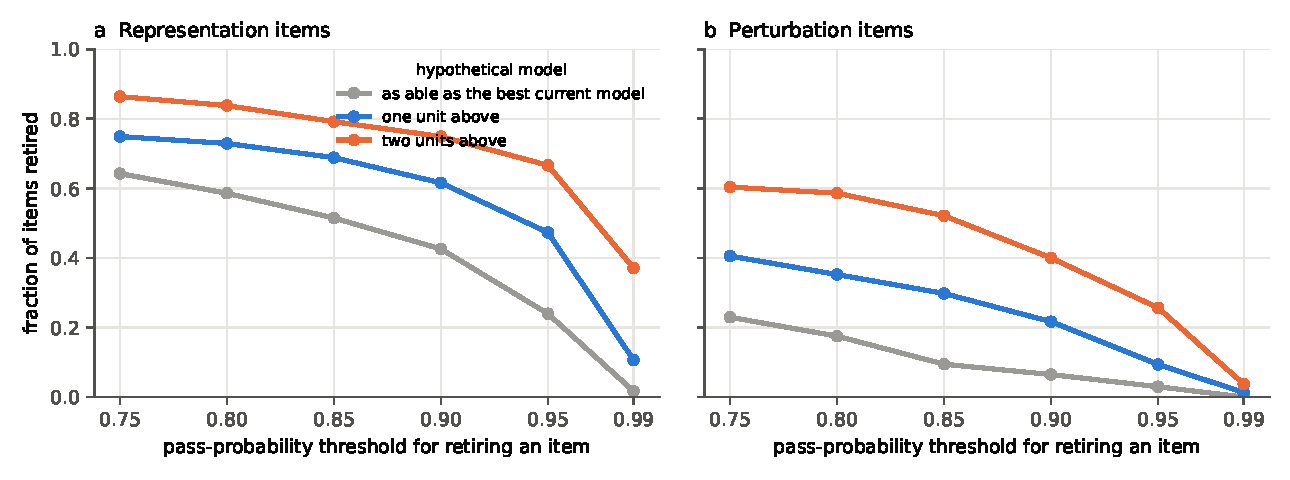
\includegraphics[width=0.55\textwidth]{fig_retire.pdf}
\caption{Fraction of informative items that a hypothetical model retires, as a function of
its ability above the best current respondent. An item is retired when the model's pass
probability reaches 0.95. Items passed by none or all current respondents are excluded
from the denominator.}
\label{fig:retire}
\end{figure}

\paragraph{Limits of this release.}
Item standard errors are 0.5 to 0.6 logits because the pool has 20 to 30
respondents; the design target of 50 to 100 halves them. The pooled perturbation
scale carries a dataset factor of 2.7 logits that linking through shared
perturbations must remove before cross-dataset difficulties are compared. The
compounds in sciPlex3 and McFarland lack chemical structures in their source files,
so those screens run only in the unseen-context setting. No pretrained foundation
model has yet been placed on the perturbation scale; that step, with a record of
which items each model has seen in pretraining, is what the scale was built for.


\begin{thebibliography}{99}
\small
\bibitem{lord1980} F.~M. Lord. \emph{Applications of Item Response Theory to Practical Testing Problems}. Erlbaum, 1980.
\bibitem{tabulasapiens2} The Tabula Sapiens Consortium. Tabula Sapiens 2.0: a comprehensive transcriptomic atlas of human cell types. \emph{Cell}, 2026 (bioRxiv 2024).
\bibitem{scperturb} S.~Peidli et al. scPerturb: harmonized single-cell perturbation data. \emph{Nature Methods}, 2024.
\bibitem{tahoe} J.~Zhang et al. Tahoe-100M: a giga-scale single-cell perturbation atlas. bioRxiv, 2025.
\bibitem{systema} Systema: assessing systematic variation in perturbation-response prediction. \emph{Nature Biotechnology}, 2025. [fill authors]
\bibitem{perturbench} Y.~Wu et al. PerturBench: benchmarking machine learning models for cellular perturbation analysis. NeurIPS Datasets and Benchmarks, 2025.
\bibitem{ahlmann2025} C.~Ahlmann-Eltze, W.~Huber, S.~Anders. Deep-learning-based gene perturbation effect prediction does not yet outperform simple linear baselines. \emph{Nature Methods}, 2025.
\bibitem{scvi} R.~Lopez et al. Deep generative modeling for single-cell transcriptomics. \emph{Nature Methods}, 2018.
\bibitem{scgen} M.~Lotfollahi, F.~A. Wolf, F.~J. Theis. scGen predicts single-cell perturbation responses. \emph{Nature Methods}, 2019.
\bibitem{kedzierska2025} K.~Z. Kedzierska et al. Zero-shot evaluation reveals limitations of single-cell foundation models. \emph{Genome Biology}, 2025.
\bibitem{souza2026} Parameter-free representations outperform single-cell foundation models on downstream benchmarks. arXiv:2602.16696, 2026. [fill authors]
\bibitem{morgan} D.~Rogers, M.~Hahn. Extended-connectivity fingerprints. \emph{J. Chem. Inf. Model.}, 2010.
\bibitem{vcc2026} Arc Institute. Virtual Cell Challenge 2026: benchmarking zero-shot generalization across cellular contexts. \emph{Cell}, 2026.
\bibitem{companion} Companion paper: Maintaining a living benchmark with item response theory. In preparation.
\end{thebibliography}

\end{document}
